% =============================================================================
% Graphical abstract as submitted (07_manuscript/as_submitted/Graphical_abstract.pdf)
% Reuses the two map panels of the pipeline output 07_manuscript/Graphical_abstract.pdf
% (written by 06_publication_figures.R) and replaces all of its text with plain-language
% wording: title, subtitle, panel titles, legends and the map-boundary note.
% Compile from the repository root:
%   pdflatex -output-directory=07_manuscript/as_submitted 00_documentation/graphical_abstract.tex
% The typology counts in the legend (27, 11, 11, 26) are typed in by hand; update
% them if a new run changes the typologies. In the submitted file, the text hidden
% by the clipping was also removed from the embedded panels (no visible effect).
% =============================================================================
\documentclass[border=0pt]{standalone}
\usepackage[T1]{fontenc}
\usepackage{helvet}
\renewcommand{\familydefault}{\sfdefault}
\usepackage{graphicx}
\usepackage{tikz}
\usepackage{array}
\definecolor{critical}{HTML}{7F0000}
\definecolor{climexp}{HTML}{F46D43}
\definecolor{servgap}{HTML}{4575B4}
\definecolor{resil}{HTML}{91CF60}
\definecolor{hot05}{HTML}{EF8A62}
\definecolor{hot10}{HTML}{FDDBC7}
\definecolor{notsig}{HTML}{F0F0F0}
\definecolor{cold10}{HTML}{D1E5F0}
\definecolor{cold05}{HTML}{67A9CF}
\definecolor{swatchline}{HTML}{8C8C8C}
\definecolor{note}{HTML}{555555}
\begin{document}
\begin{tikzpicture}[x=1bp,y=1bp]
\path[use as bounding box] (0,0) rectangle (720,331);

% ---- Title and subtitle -----------------------------------------------------
\node[anchor=north west, inner sep=0, font=\bfseries\fontsize{15}{18}\selectfont]
  at (12,322) {Where harsh climate meets weak access to services in Morocco};
\node[anchor=north west, inner sep=0, text width=696bp, align=left,
      font=\fontsize{10}{12.5}\selectfont]
  at (12,300) {An open-data index for Morocco's 75 provinces shows that harsh climate and weak access to roads and services occur together mainly in the south and interior.};

% ---- Panel titles -----------------------------------------------------------
\node[anchor=north west, inner sep=0, font=\bfseries\fontsize{11}{13}\selectfont]
  at (12,266) {Four planning types};
\node[anchor=north west, inner sep=0, font=\bfseries\fontsize{11}{13}\selectfont]
  at (372,266) {Where high and low scores cluster};

% ---- Maps (cropped from the pipeline figure, scaled to 90%) -----------------
\node[anchor=south west, inner sep=0] at (8,20)
  {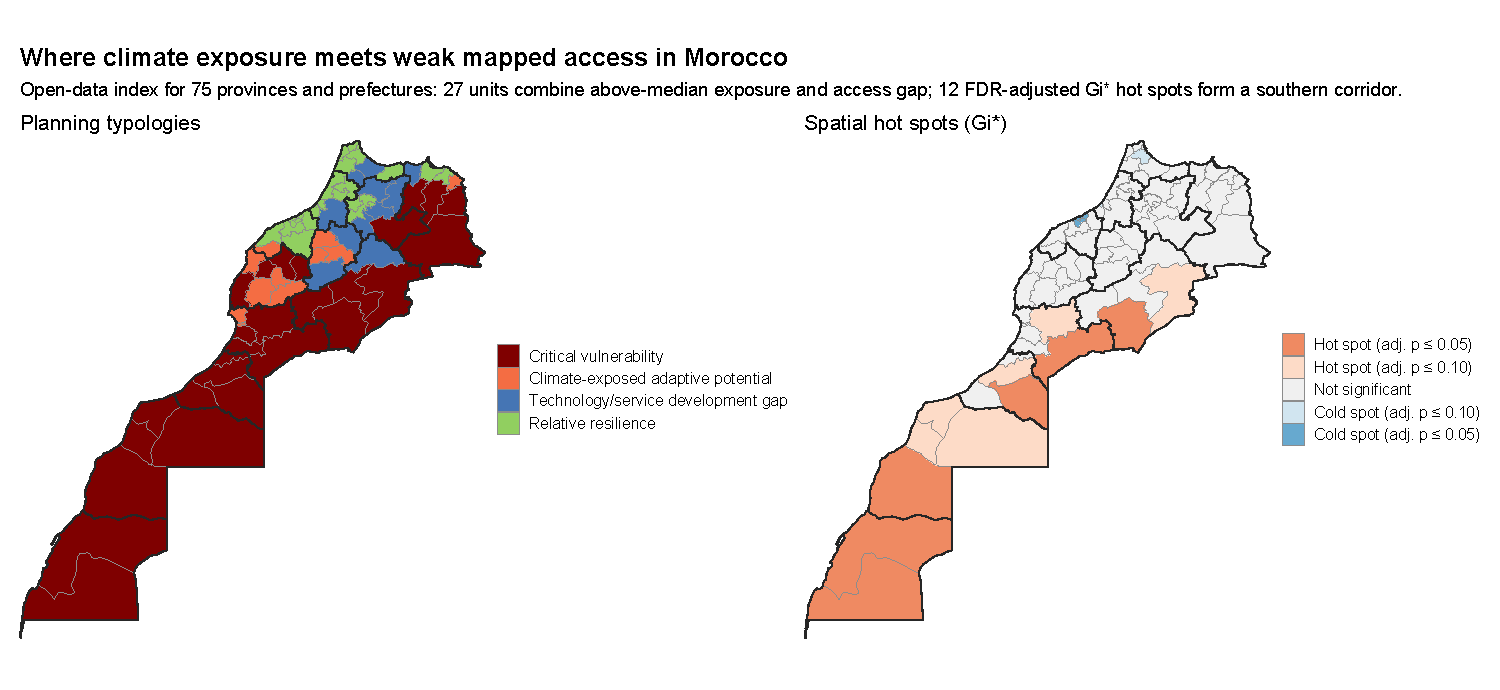
\includegraphics[scale=0.9, trim=9 24.5 487 67, clip]{07_manuscript/Graphical_abstract.pdf}};
\node[anchor=south west, inner sep=0] at (368,20)
  {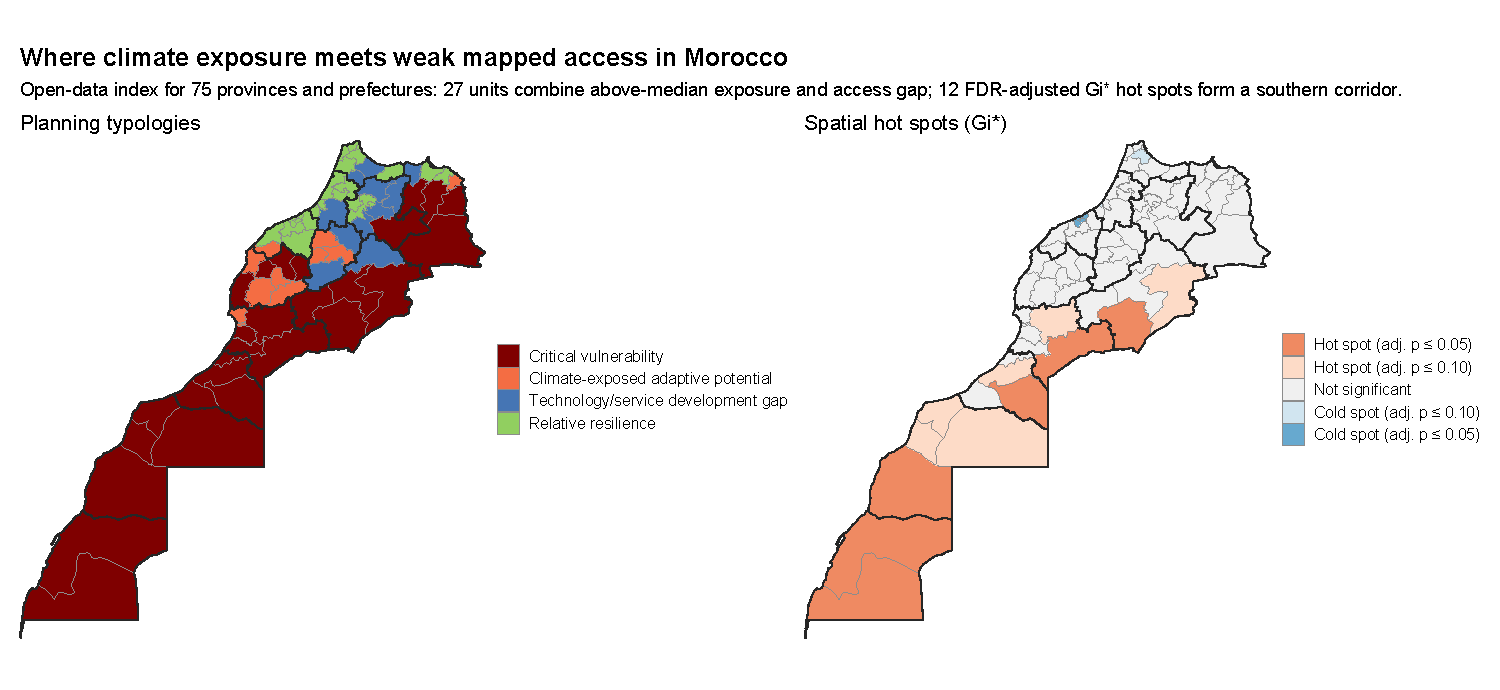
\includegraphics[scale=0.9, trim=385.5 24.5 110 67, clip]{07_manuscript/Graphical_abstract.pdf}};

% ---- Legend: planning types -------------------------------------------------
\newcommand{\swatch}[1]{\tikz[baseline=-1bp]\fill[#1, draw=swatchline, line width=0.4bp] (0,-4) rectangle (10,6);}
\newcommand{\typeentry}[3]{\swatch{#1} & {\bfseries\fontsize{8}{9.6}\selectfont #2}\newline
  {\color{note}\fontsize{7.5}{9}\selectfont #3}\\[7bp]}
\node[anchor=west, inner sep=0] at (213,140) {%
  \hyphenpenalty=10000\exhyphenpenalty=10000
  \renewcommand{\arraystretch}{1}\setlength{\tabcolsep}{2.5bp}%
  \begin{tabular}{@{}l>{\raggedright\arraybackslash}p{132bp}@{}}
  \typeentry{critical}{Critical vulnerability (27)}{Harsh climate, weak access}
  \typeentry{climexp}{Climate-exposed adaptive potential (11)}{Harsh climate, better access}
  \typeentry{servgap}{Technology/service development gap (11)}{Milder climate, weak access}
  \typeentry{resil}{Relative resilience (26)}{Milder climate, better access}
  \end{tabular}};

% ---- Legend: clusters -------------------------------------------------------
\newcommand{\clusterentry}[3]{% y, colour, label
  \fill[#2, draw=swatchline, line width=0.4bp] (576,#1-9) rectangle (586,#1+1);
  \node[anchor=west, inner sep=0, font=\fontsize{8}{9.4}\selectfont]
    at (591,#1-4) {#3};}
\clusterentry{181}{hot05}{Hot spot: strong evidence}
\clusterentry{164}{hot10}{Hot spot: weaker evidence}
\clusterentry{147}{notsig}{No clear cluster}
\clusterentry{130}{cold10}{Cold spot: weaker evidence}
\clusterentry{113}{cold05}{Cold spot: strong evidence}
\node[anchor=north west, inner sep=0, text width=128bp, align=left,
      font=\fontsize{7.5}{9}\selectfont, text=note]
  at (576,98) {Hot spots are groups of neighbouring provinces with high scores; cold spots have low scores.};

% ---- Footnote ---------------------------------------------------------------
\node[anchor=south west, inner sep=0, font=\fontsize{6.5}{8}\selectfont, text=note]
  at (12,5) {Map lines delineate study areas and do not necessarily depict accepted national boundaries.};
\end{tikzpicture}
\end{document}
